\documentclass[a4paper,11pt]{article}

% Geometry for page layout
\usepackage[a4paper, top=1in, bottom=1in, left=1in, right=1in]{geometry}

%% line spacing %%
\renewcommand{\baselinestretch}{1.1}

\usepackage{amsmath, amssymb, amsthm}
\usepackage{bm} % Bold math symbols
\usepackage{mathtools} % Additional math symbols
\usepackage{enumitem} % Customizable lists
% \usepackage{marvosym} & \Lightning

% Font and styling
\usepackage{lmodern}
\usepackage{mdframed}
\usepackage{titlesec}
\usepackage{url}
\usepackage{xcolor}
\usepackage{graphicx}
\usepackage{fancyhdr, bbm}
\usepackage{parskip} % Spacing between paragraphs

\mdfdefinestyle{commandline}{
	leftmargin=5pt,
	rightmargin=5pt,
	innerleftmargin=15pt,
	innertopmargin = 9pt,
	innerbottommargin = 9pt,
	middlelinecolor=black!20!white,
	middlelinewidth=1pt,
	frametitlerule=false,
	backgroundcolor=black!2!white,
	nobreak,
}

% Define a custom environment for command-line snapshots
\newenvironment{commandline}{
	\medskip
	\begin{mdframed}[style=commandline]
	}{
	\end{mdframed}
	\medskip
}


% Header and Footer
\pagestyle{fancy}
\renewcommand{\headrulewidth}{0pt}
\renewcommand{\theequation}{\Roman{equation}}
\fancyhf{} % Clear header and footer
\fancyfoot[R]{\thepage} % Right-aligned page number in the footer

\newcommand{\x}{\mathbf{x}}
\newcommand{\y}{\mathbf{y}}
\newcommand{\yhat}{\hat{\mathbf{y}}}


% Custom commands
\newcommand{\hessianmatrix}{
	\begin{bmatrix}
		\displaystyle \frac{\partial^2 f}{\partial x_1^2} & \displaystyle \frac{\partial^2 f}{\partial x_1 \partial x_2} \\[20pt]
		\displaystyle \frac{\partial^2 f}{\partial x_2 \partial x_1} & \displaystyle \frac{\partial^2 f}{\partial x_2^2}
	\end{bmatrix}
}
%todo command
\newcommand{\todo}[1]{\textcolor{red}{TODO: #1}}
%norm command
\newcommand{\norm}[1]{\| #1 \|} % Basic norm
\newcommand{\pnorm}[2]{\| #1 \|_{#2}} % p_norm with p as second arg

\begin{document}
	
	% Title block
	\begin{center}
		{\fontsize{18}{10}\selectfont \textbf{Assignment X}} \\
		\vspace{0.3cm}
		{\textbf{Subject WS24}} \\
		\vspace{0.2cm}
		\textbf{John Doe} \\
		\vspace{0.2cm}
		\today
	\end{center}
	
	\vspace{0.3cm}
	
\section{Section 1}
	
Lorem ipsum dolor sit amet, consetetur sadipscing elitr, sed diam nonumy eirmod tempor invidunt ut labore et dolore magna aliquyam.
 	\[ \frac{\partial\mathcal{L}}{\partial \mathbf{b}^{(1)}} =  
 \frac{\partial\mathcal{L}}{\partial \mathbf{a}^{(2)}} \cdot
 \frac{\partial \mathbf{a}^{(2)}}{\partial \mathbf{z}^{(2)}} \cdot
 \frac{\partial \mathbf{z}^{(2)}}{\partial \mathbf{b}^{(1)}}\]
 \[ \Rightarrow
 \frac{\partial \mathcal{L}}{\partial b_k^{(1)}} = \frac{\partial \mathcal{L}}{\partial a_i^{(2)}} \cdot \frac{\partial a_i^{(2)}}{\partial z_k^{(2)}} \cdot \frac{\partial z_k^{(2)}}{\partial b_k^{(1)}} = - \sum_{i = 1}^{3} y_i\frac{1}{a_i^{(2)}} \cdot a_i^{(2)}  (\mathbbm{1}\{i = k\}-a_k^{(2)}) \cdot 1
 \]
 \[ = - \sum_{i = 1}^{3} y_i (\mathbbm{1}\{i = k\}-a_k^{(2)}) = - \sum_{i = 1}^{3} y_i\mathbbm{1}\{i = k\}-y_ia_k^{(2)} = \sum_{i = 1}^{3}y_ia_k^{(2)} - \sum_{i = 1}^{3} y_i\mathbbm{1}\{i = k\} \]
 
\section{Sec 2}

\subsection{Subsection}

 For a random sample from the batch we achieve the following results:
\begin{commandline}
	\begin{verbatim}
Some code or results...
	\end{verbatim}
\end{commandline}
	\begin{figure}[!h]
	\centering
	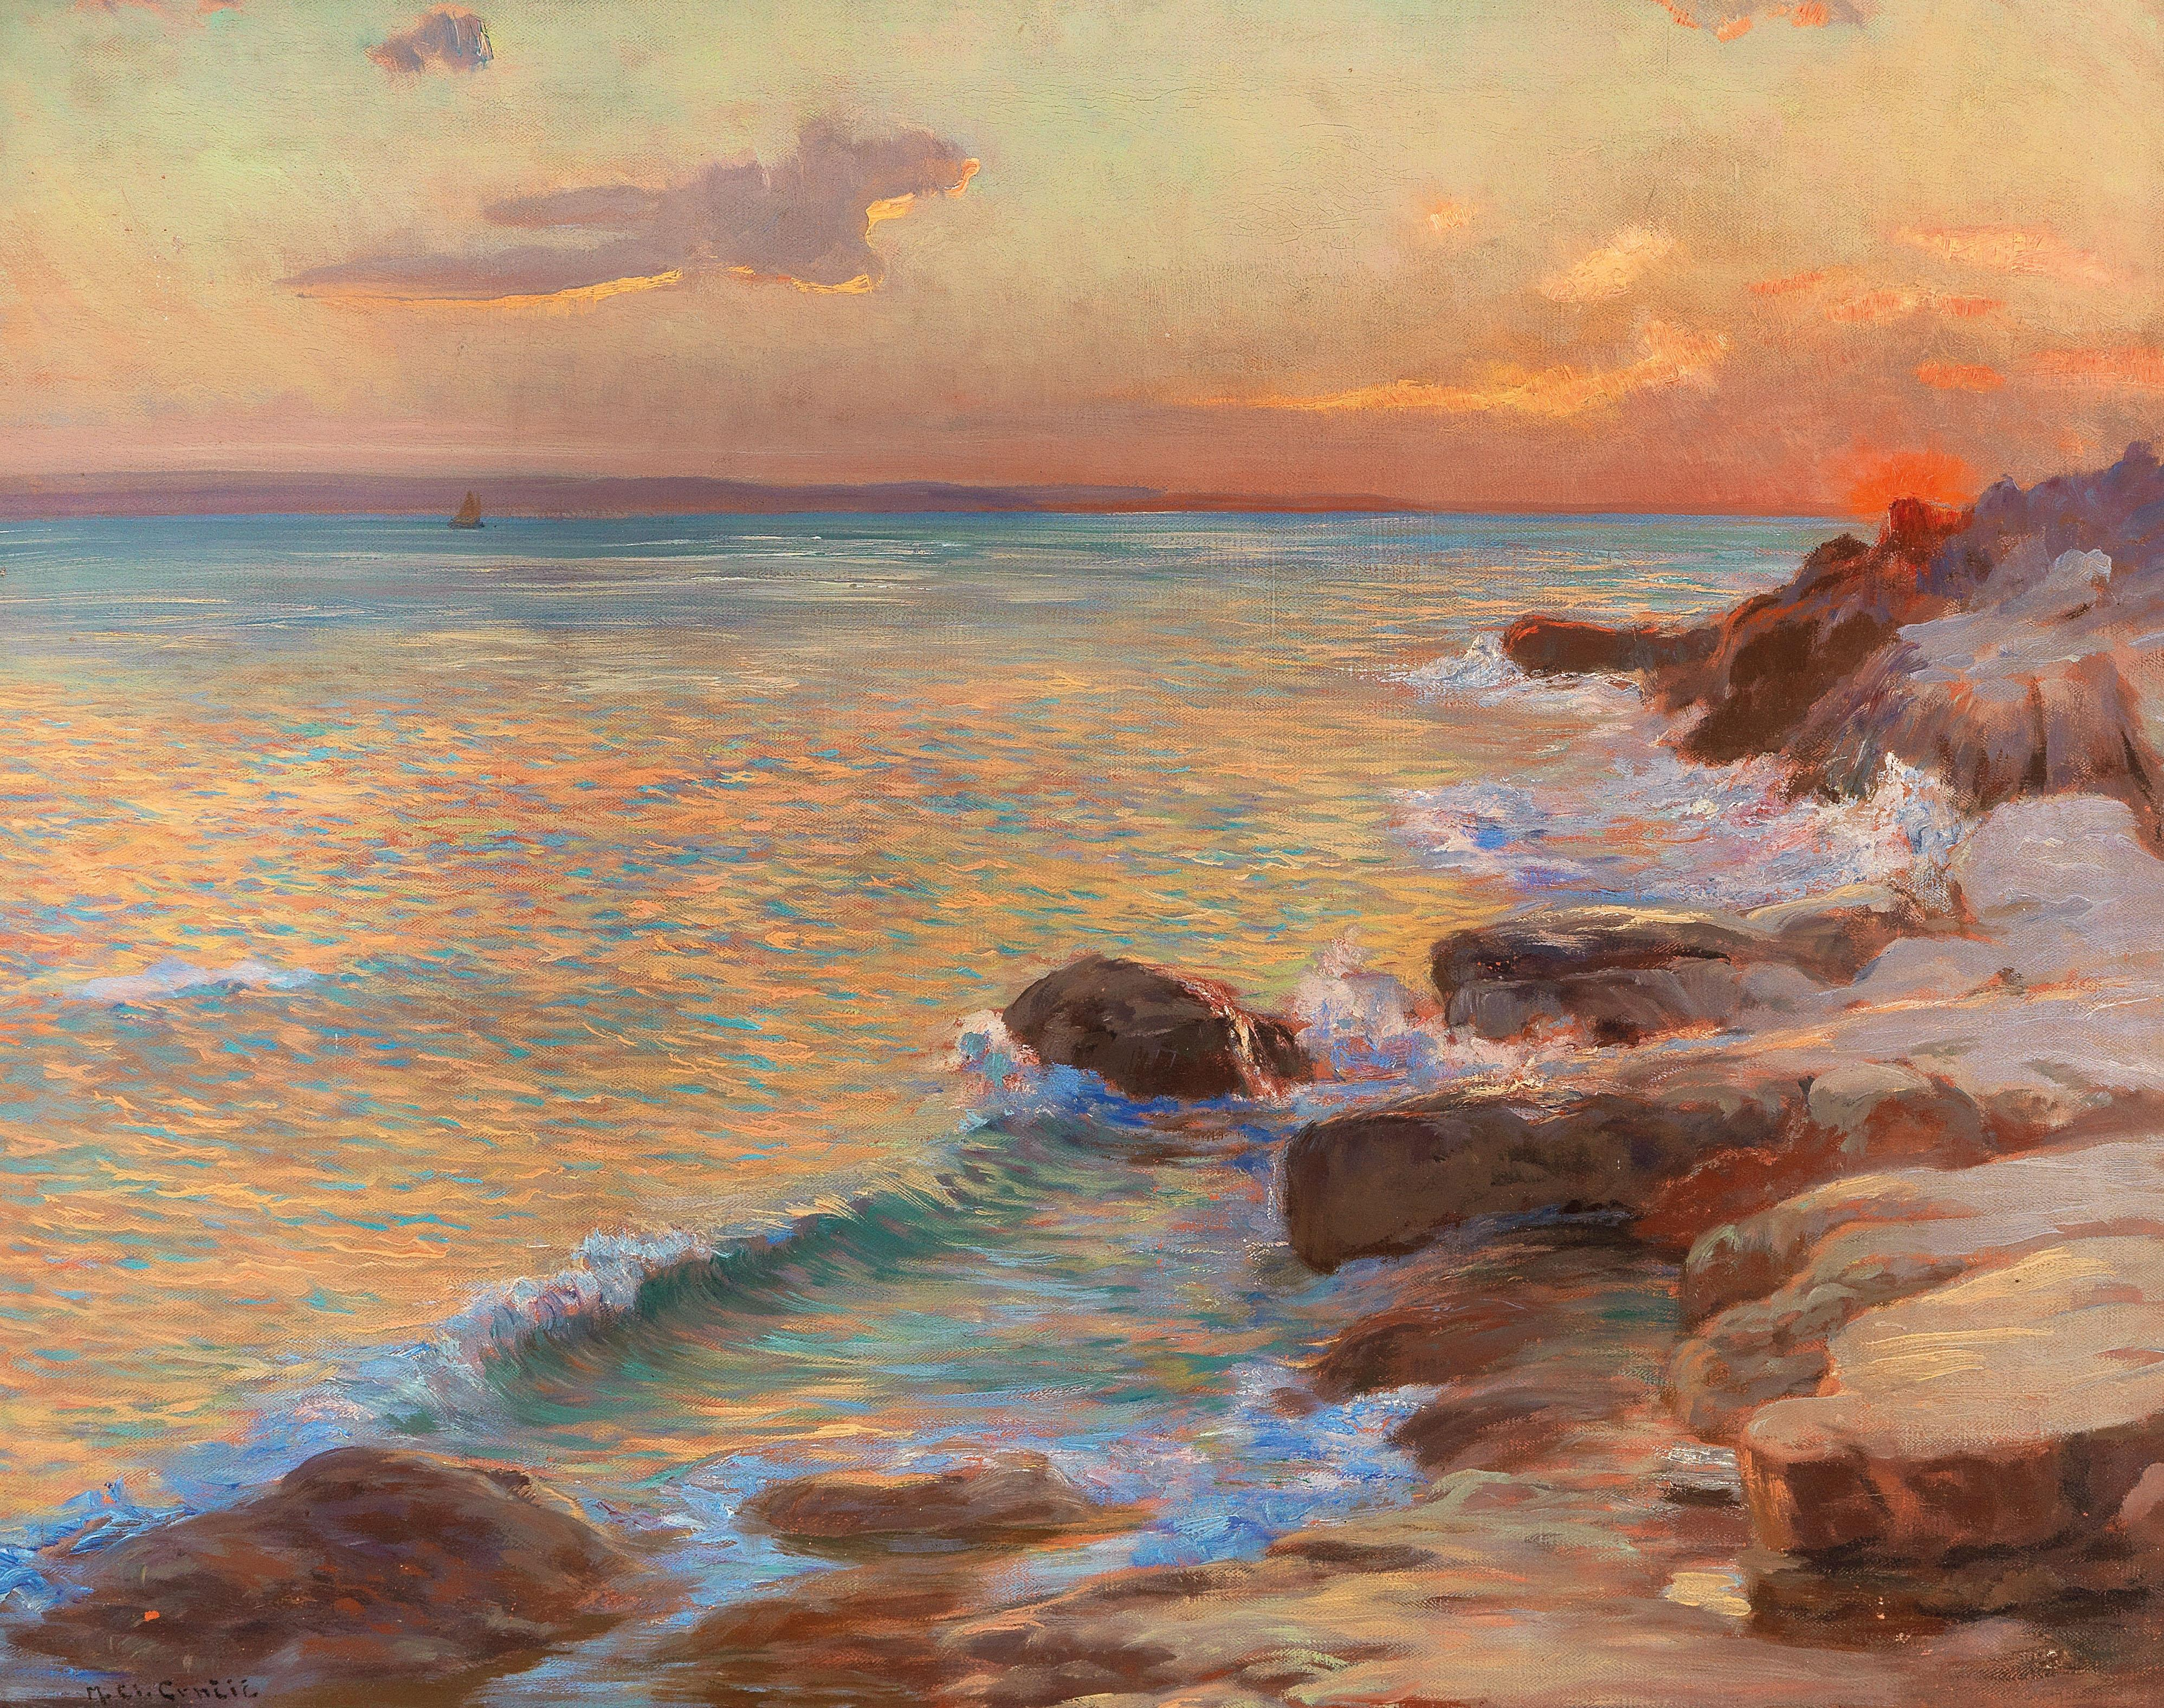
\includegraphics[width=0.5\linewidth]{sunset_in_split}
	\label{fig:enter-label}
	\caption{Sunset in Split by Menci Clement Crnčić (1930)}
\end{figure}

 
\end{document}
